\documentclass{article}
\usepackage[utf8]{inputenc}
\usepackage[margin=1in,left=1in,includefoot]{geometry}
\usepackage{graphicx}  % allows to add images
\usepackage{times} % Times New Roman font
\usepackage{titlesec} % For redefining \paragraph
\usepackage{float}
% Header & Footer Stuff

\usepackage{fancyhdr}
\pagestyle{fancy}
\lhead{COL334 : Computer Networks}
\rhead{}
\fancyfoot{}
\fancyfoot[R]{}

\titlespacing{\paragraph}{0pt}{0pt}{1em}


\begin{document}

\begin{center}
 \LARGE\bfseries Assignment 1 Part 1
\end{center}

\section{Ping}


\normalsize
To ping \textit{google.com} and \textit{sigcomm.com} 10 times using two different networks.
We ping both the websites on IIT Delhi's network and Cellular network through mobile's personal hotspot.

\subsubsection*{Google.com}

\begin{figure}[H]
    \centering
    \begin{minipage}{0.5\textwidth}
        \centering
        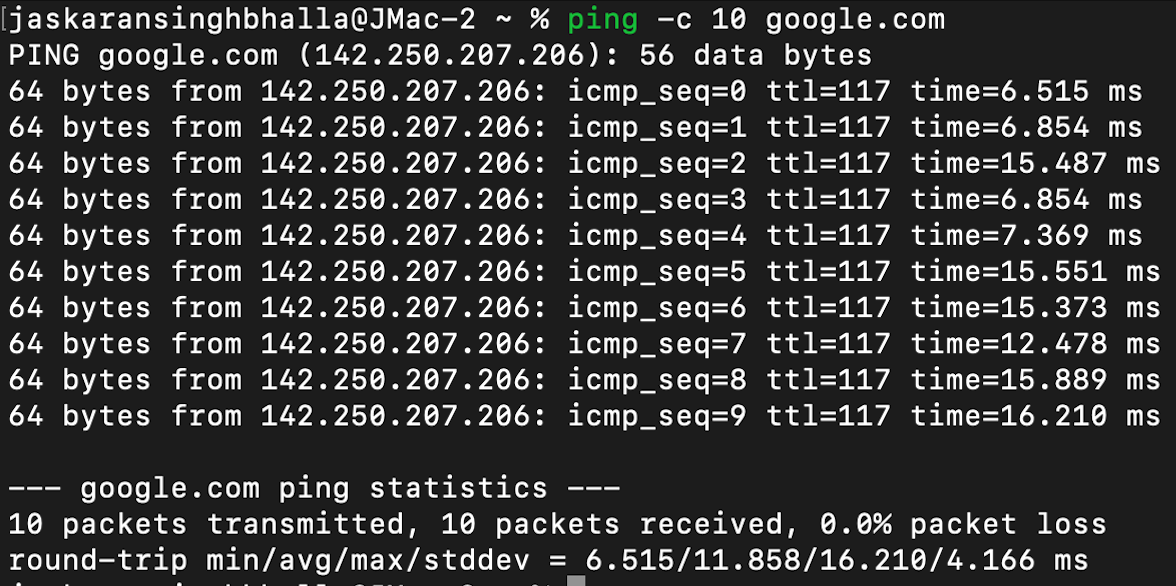
\includegraphics[width=\linewidth]{part-1/ping-google-iitd.png}
        \caption{IIT Delhi Network}
    \end{minipage}
    \hfill
    \begin{minipage}{0.45\textwidth}
        \centering
        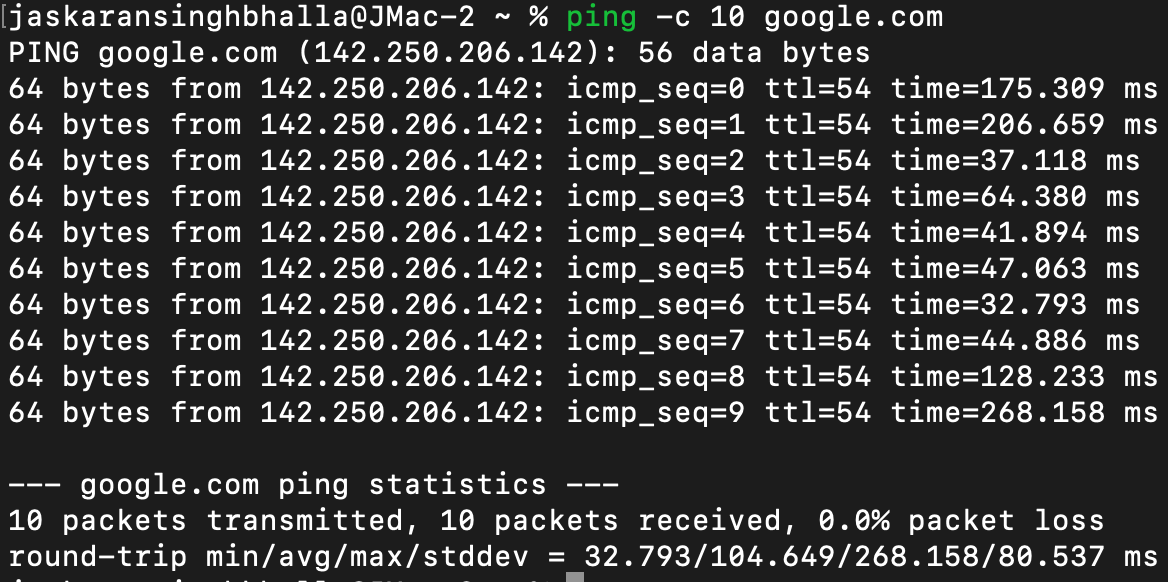
\includegraphics[width=\linewidth]{part-1/ping-google-hotspot.png}
        \caption{Cellular Network using Hotspot}
    \end{minipage}
\end{figure}

\subsubsection*{Sigcomm.org}

\begin{figure}[H]
    \centering
    \begin{minipage}{0.45\textwidth}
        \centering
        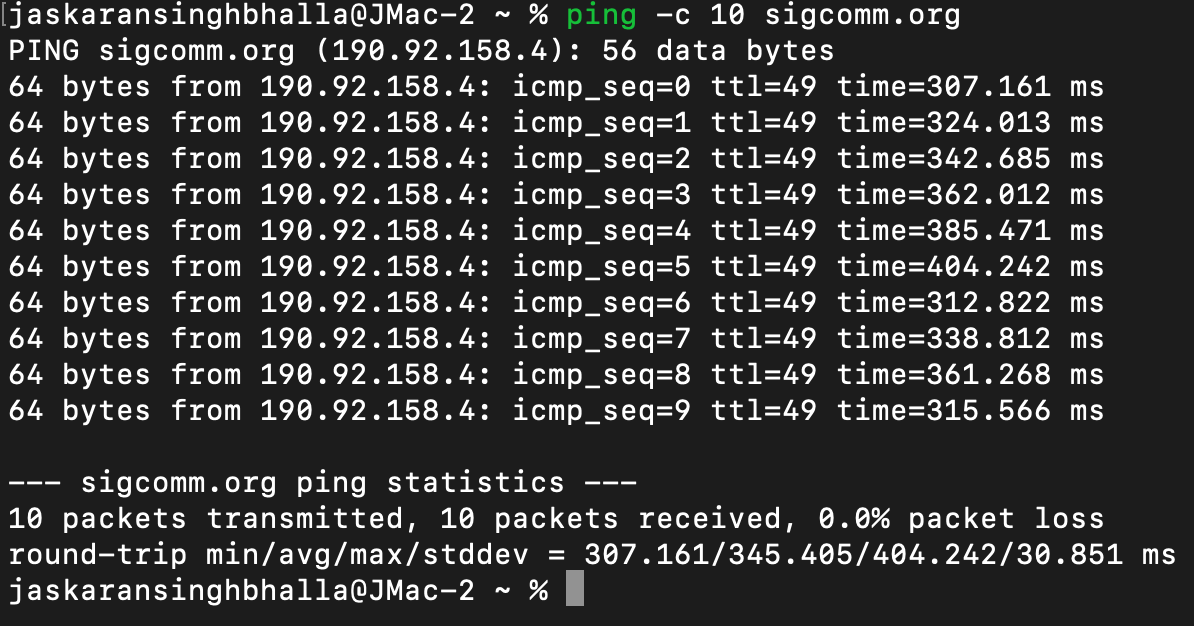
\includegraphics[width=\linewidth]{part-1/ping-sigcomm-iitd.png}
        \caption{IIT Delhi Network}
    \end{minipage}
    \hfill
    \begin{minipage}{0.45\textwidth}
        \centering
        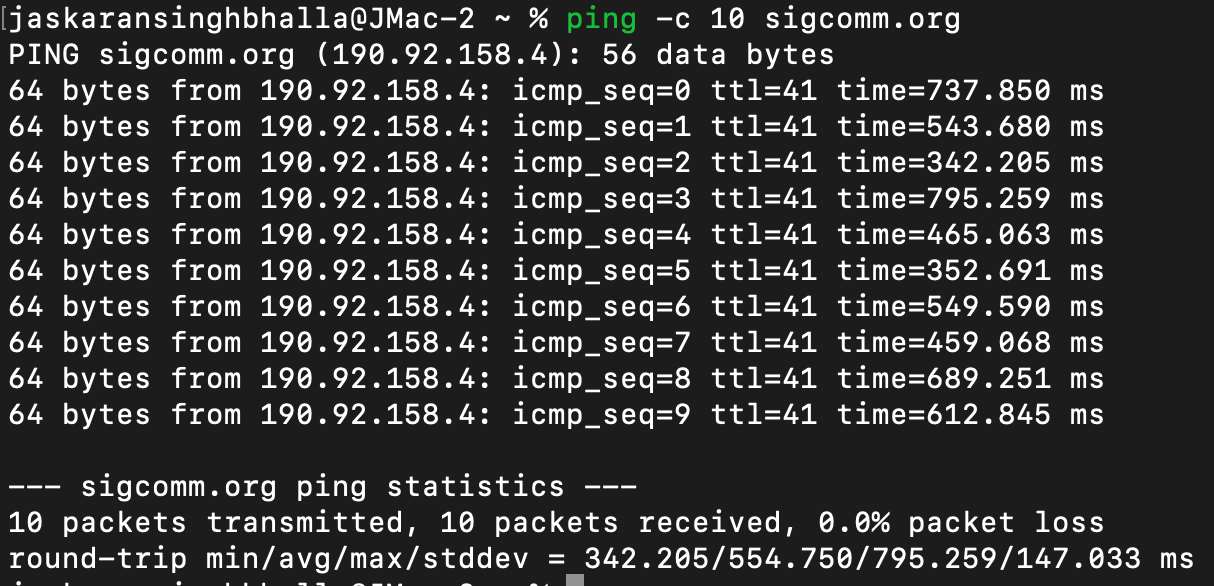
\includegraphics[width=\linewidth]{part-1/ping-sigcomm-hotspot.png}
        \caption{Cellular Network using Hotspot}
    \end{minipage}
\end{figure}

\subsection{Comparison of the Ping Latency}

Ping latency is a measure of the time taken by a signal (a data packet) to travel from a source to a destination and back again. This round-trip time is measured in milliseconds (ms). 

\subsubsection{Different websites on the same network}

\normalsize
We can observe that the average ping for \textit{google.com} is 11.858 ms and the average ping for \textit{sigcomm.org} is 345.405 ms on IIT Delhi's Network. 

\normalsize
Similarly the average ping for \textit{google.com} is 104.649 ms and the average ping for \textit{sigcomm.com} is 554.750 ms on cellular network. It is clearly observed that the average ping for \textit{google.com} is greater than \textit{sigcomm.com} for both the networks. 

% Reason Pending

\subsubsection{Same website on different networks}

\paragraph{
\normalsize
The average ping for \textit{google.com} is 11.858 ms  on IIT Delhi's network and is 104.649 ms on cellular network. 
}
\paragraph{
\normalsize
The average ping for \textit{sigcomm.com} is 345.405 ms  on IIT Delhi's network and is 554.750 ms ms on cellular network. 
}

\paragraph{}
\normalsize
We can see that the ping is different for same website on different networks. One possible reason for it could be the bandwidth of the network or the speed of the network.
% Reason Pending

\subsection{Protocol related questions}
\subsubsection{ICMP Protocol}
\normalsize
\noindent
Ping command uses ICMP (Internet Control Message Protocol) to send a request and obtain the response from the gateway or host. It sends packets as Echo request to the server and pings the server to test it's availability and it return gets an Echo response. It measures the round trip time between the host and the destination. A typical ICMP response consits of ICMP echo reply packet, RTT(Round-Trip Time), Packet loss, TTL (Time To Live), Response Size and Sequence number. This protocol is a network layer protocol and is important for error reporting and testing. It is implemented in routers. This protocol doesn't require a handshake in order to be executed, so it's a connection less protocol.

\subsubsection{Theoretical Upper limit on packet size}
\normalsize
\noindent
In order to determine theoretical upper limit of packet size for the ping protocol, we need to understand what the packet size depends on and understand a typical ICMP packet. ICMP packets include an ICMP header after a normal IP header. IPv4 and IPv6 are two versions of Internet Protocol (IP) that are used commonly and they have different size for the headers. ICMP header comes after IPv4 and IPv6 packet header. The theoretical upper limit of the packet size for the ping protocol is determined by the underlying network protocol, which is typically IPv4 or IPv6. Size of IPv4 header is 20 bytes and IPv6 header is 40 bytes. Size of ICMP header is 8 bytes. This size can further increase based upon the options used.\\

\noindent
Upper limit on the packet size on internet is determined by Maximum Transmission Unit (MTU) of the network resources. Theoretically, the maximum packet size, or Maximum Transmission Unit (MTU), for an IPv4 packet is 65,535 bytes. However, this includes the IPv4 header (typically 20 bytes without options) and the ICMP header (8 bytes). Therefore, the maximum ICMP payload size for an IPv4 packet is 65,507 bytes (65,535 - 20 - 8). The maximum packet size for an IPv6 packet is also 65,535 bytes. The IPv6 header is 40 bytes, and the ICMP header is 8 bytes, resulting in a maximum ICMP payload size of 65,487 bytes (65,535 - 40 - 8).\\
\textbullet{} IPv4: Theoretical maximum ICMP payload size is 65,507 bytes.\\
\textbullet{} IPv6: Theoretical maximum ICMP payload size is 65,487 bytes.

\subsubsection{Ping the websites at maximum theoretical limit}

\noindent
We try to ping \textit{google.com} using max limit for IPv4. By default when we use \verb|ping| commend, it pings the destination using IPv4 protocol.\\

\noindent
Here's a screenshot showing the output when we ping at the theoretical max value.\\
\begin{figure}[H]
    \centering
    \begin{minipage}{0.45\textwidth}
        \centering
        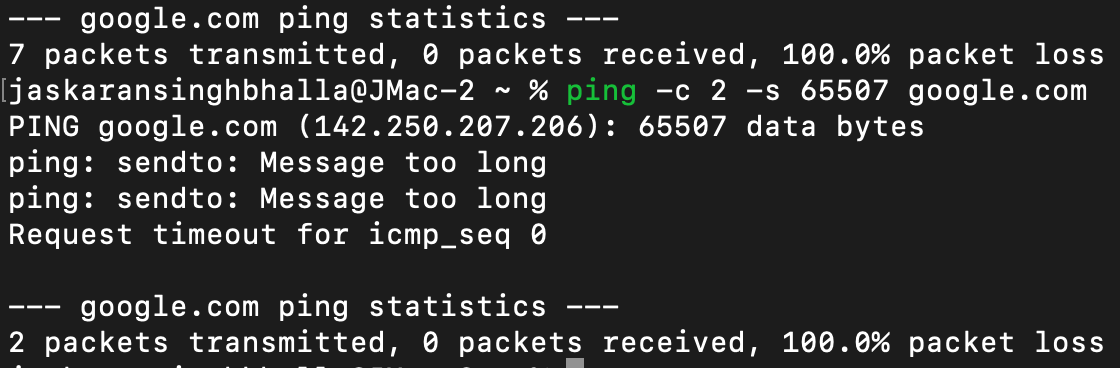
\includegraphics[width=\linewidth]{part-1/ping-theoretical-max.png}
    \end{minipage}
\end{figure}


\noindent
Generally, the packet size gets restricted by the Maximum Transmission Unit (MTU) of network resources. Practically the MTU of Ethernet and WLAN (Wifi) is around ~1500 bytes. Due to this we are not able to ping at the maximum theoretical value. Also the value gets decreased based upon the options provided in the headers.\\ 
So, due to common MTU settings, practical ICMP payload sizes are:\\
\textbullet{} IPv4: 1,472 bytes.\\
\textbullet{} IPv6: 1,452 bytes.\\

\subsection{Forcing the networks to ping using IPv6 protocol}

\noindent
We can ping the networks using IPv6 protocol using, \verb|ping6| command. It forces ping using v6 IP protocol.
Some networks might not fully support IPv6 or might have specific configurations that affect how IPv6 addresses are resolved. For instance, corporate or private networks might have restrictions or specific settings that affect IPv6 connectivity.

\subsubsection*{Google.com}

\begin{figure}[H]
    \centering
    \begin{minipage}{0.5\textwidth}
        \centering
        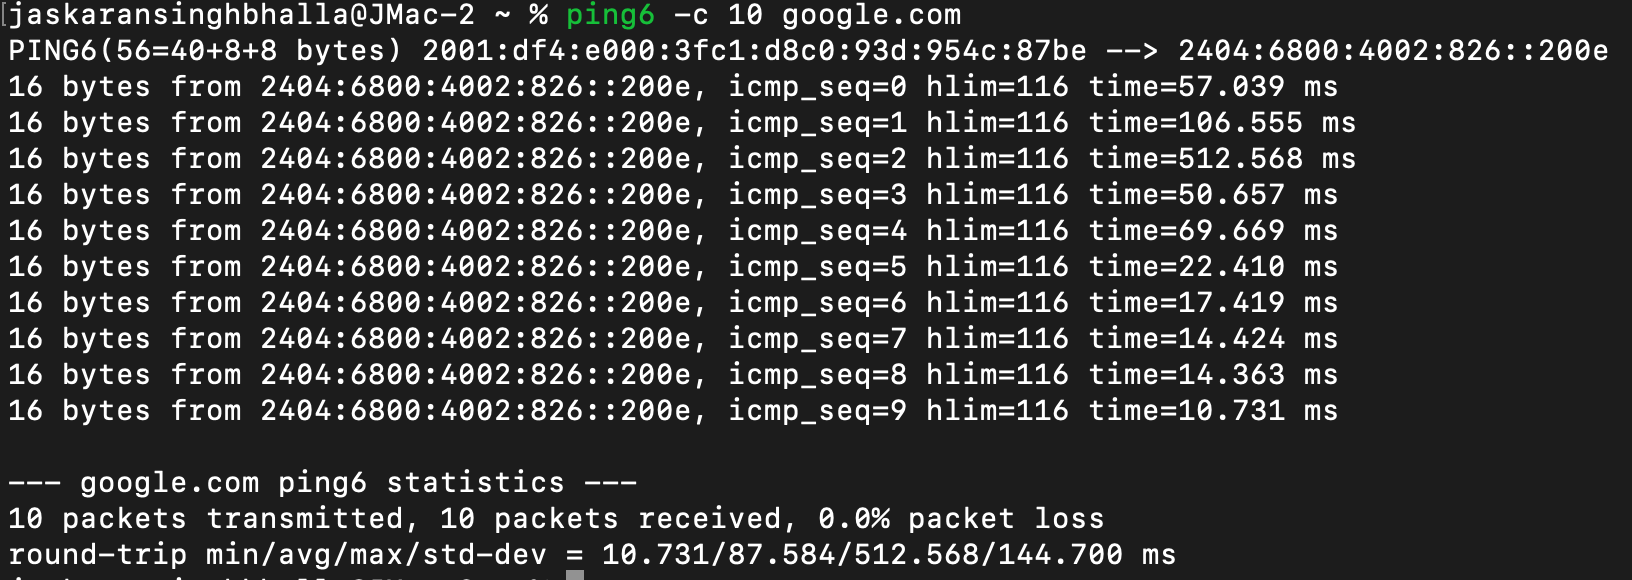
\includegraphics[width=\linewidth]{part-1/ping-ipv6-google-iitd.png}
        \caption{IIT Delhi Network}
    \end{minipage}
    \hfill
    \begin{minipage}{0.45\textwidth}
        \centering
        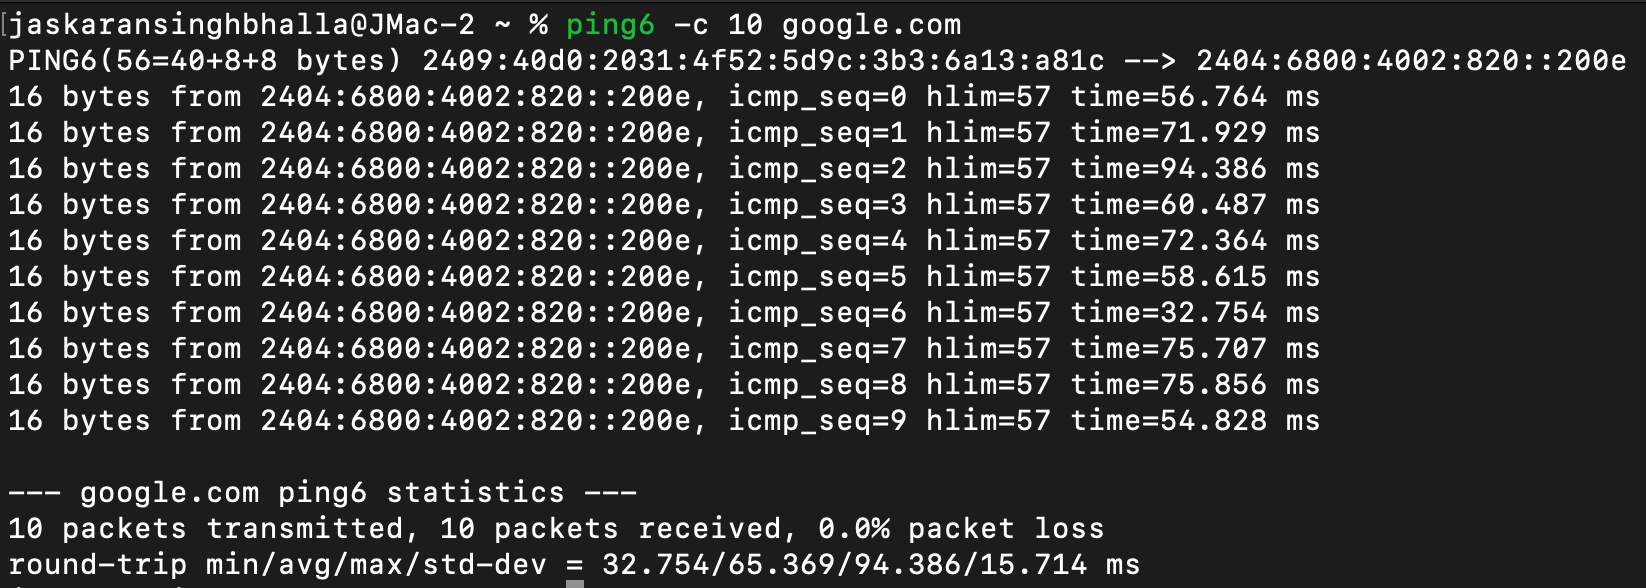
\includegraphics[width=\linewidth]{part-1/ping-ipv6-google-cellular.png}
        \caption{Cellular Network using Hotspot}
    \end{minipage}
\end{figure}

\subsubsection*{Sigcomm.org}

\begin{figure}[H]
    \centering
    \begin{minipage}{0.45\textwidth}
        \centering
        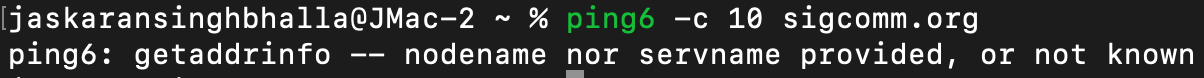
\includegraphics[width=\linewidth]{part-1/ping-ipv6-sigcomm-iitd.png}
        \caption{IIT Delhi Network}
    \end{minipage}
    \hfill
    \begin{minipage}{0.45\textwidth}
        \centering
        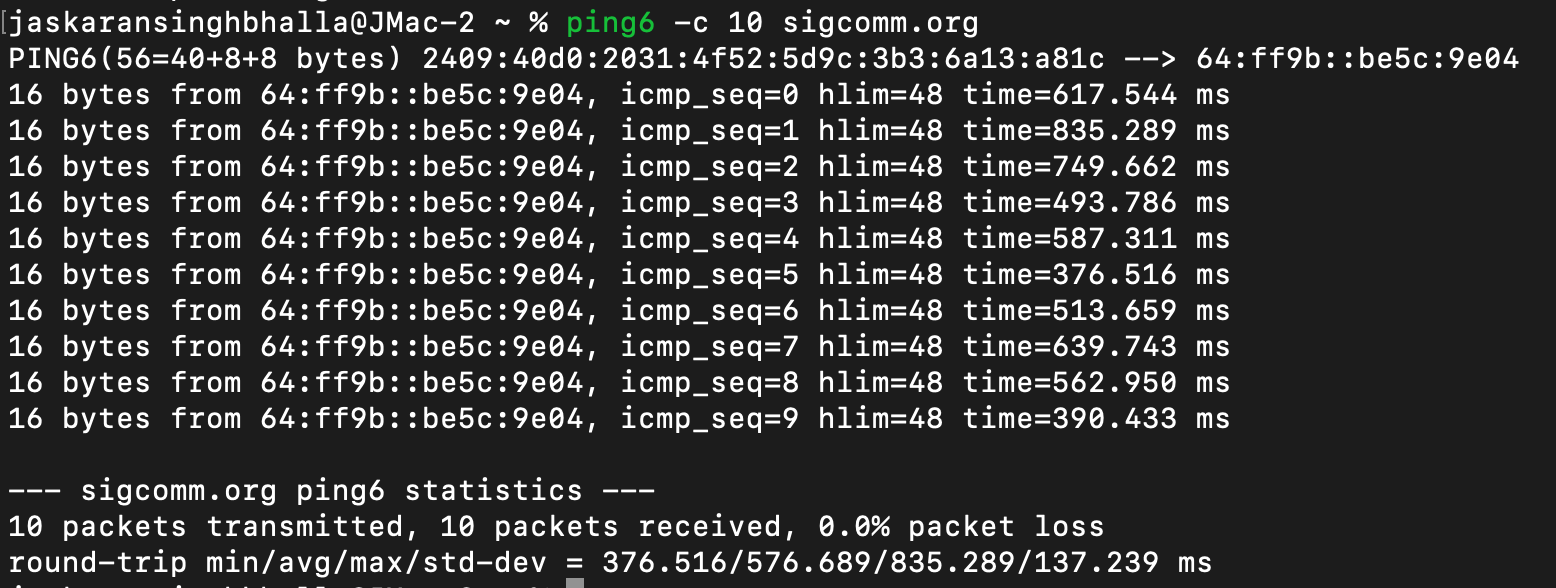
\includegraphics[width=\linewidth]{part-1/ping-ipv6-sigcomm-cellular.png}
        \caption{Cellular Network using Hotspot}
    \end{minipage}
\end{figure}

\noindent
The above screenshots show the result of ping on \textit{google.com} and \textit{sigcomm.org} using IIT Delhi's network and cellular network. The ping6 request succeeds for most of the cases, but it failed for \textit{sigcomm.org} using IIT Delhi's network. There can be multiple reasons that may cause this. It is possible that the domain for \textit{sigcomm.org} doesn't have an IPv6 address. This can be verified using \verb|nslookup -type=AAAA| and this command verifies that the \textit{sigcomm.org} does have an IPv6 address, which is also confirmed by the fact that we are able to ping it using IPv6 request on cellular network. This brings us to the conclusion, that IIT Delhi's Wifi network has some restrictions or maybe it lacks somewhere due to which it is not able to ping this address. This is often the case in private or enterprise organizations as some networks might not fully support IPv6 or might have specific configurations that affect how IPv6 addresses are resolved. For instance, corporate or private networks might have restrictions or specific settings that affect IPv6 connectivity. So this might be the reason for failure.

\section{Trace route}

\subsection{Logging Server IPs and Packet paths}

\noindent
We used \verb|nslookup| to log the server IP address of both the websites hosts on the IIT Delhi's network and Cellular network via hotspot . Then we have used \verb|traceroute| command to log the path taken by the packets.

\subsubsection*{Google.com}

\begin{figure}[H]
    \centering
    \begin{minipage}{0.5\textwidth}
        \centering
        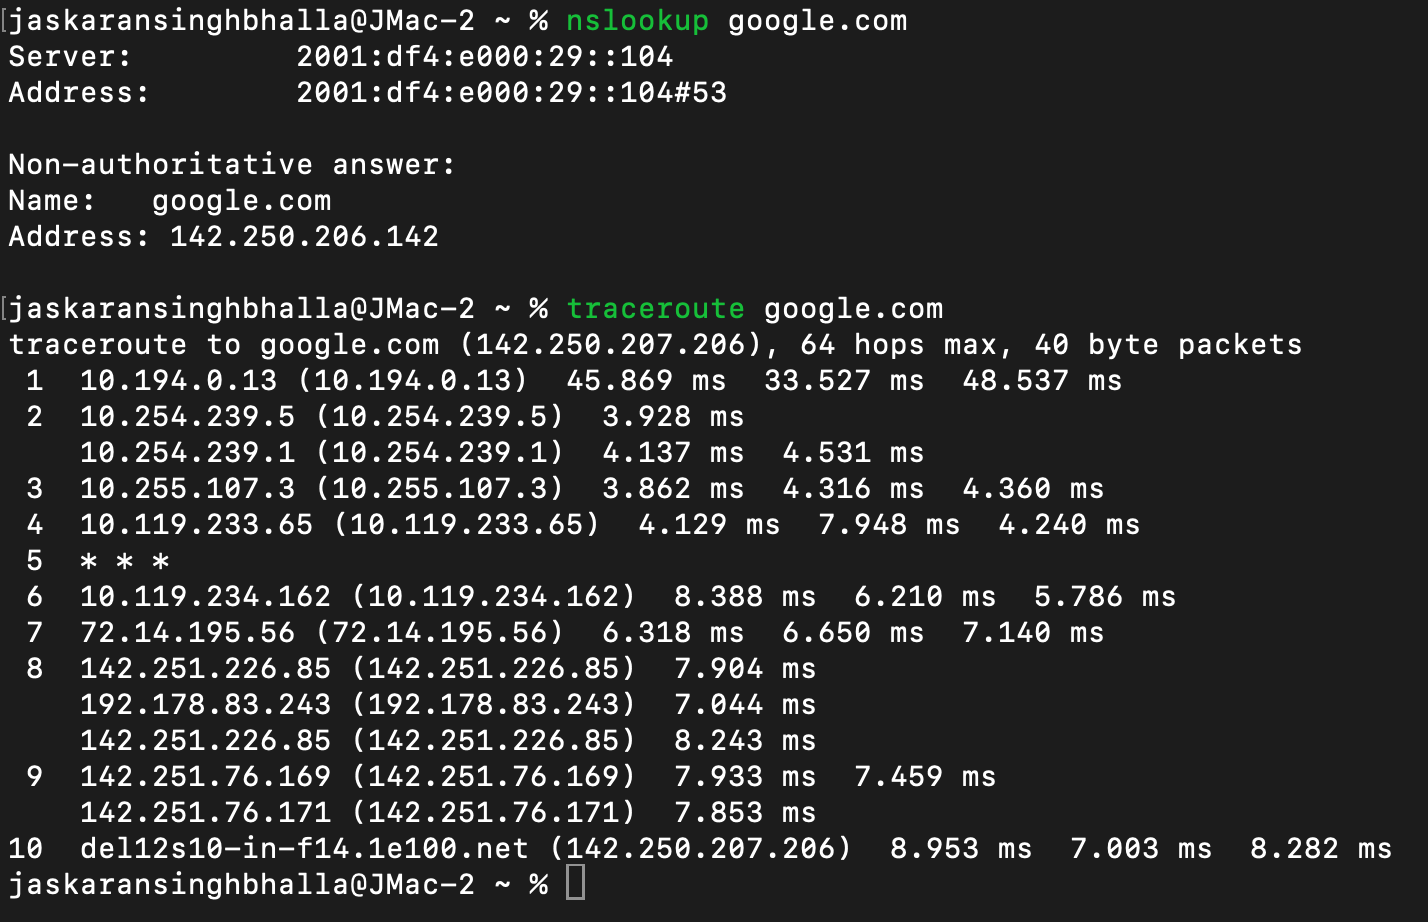
\includegraphics[width=\linewidth]{part-1/traceroute-iitd-google.png}
        \caption{IIT Delhi Network}
    \end{minipage}
    \hfill
    \begin{minipage}{0.45\textwidth}
        \centering
        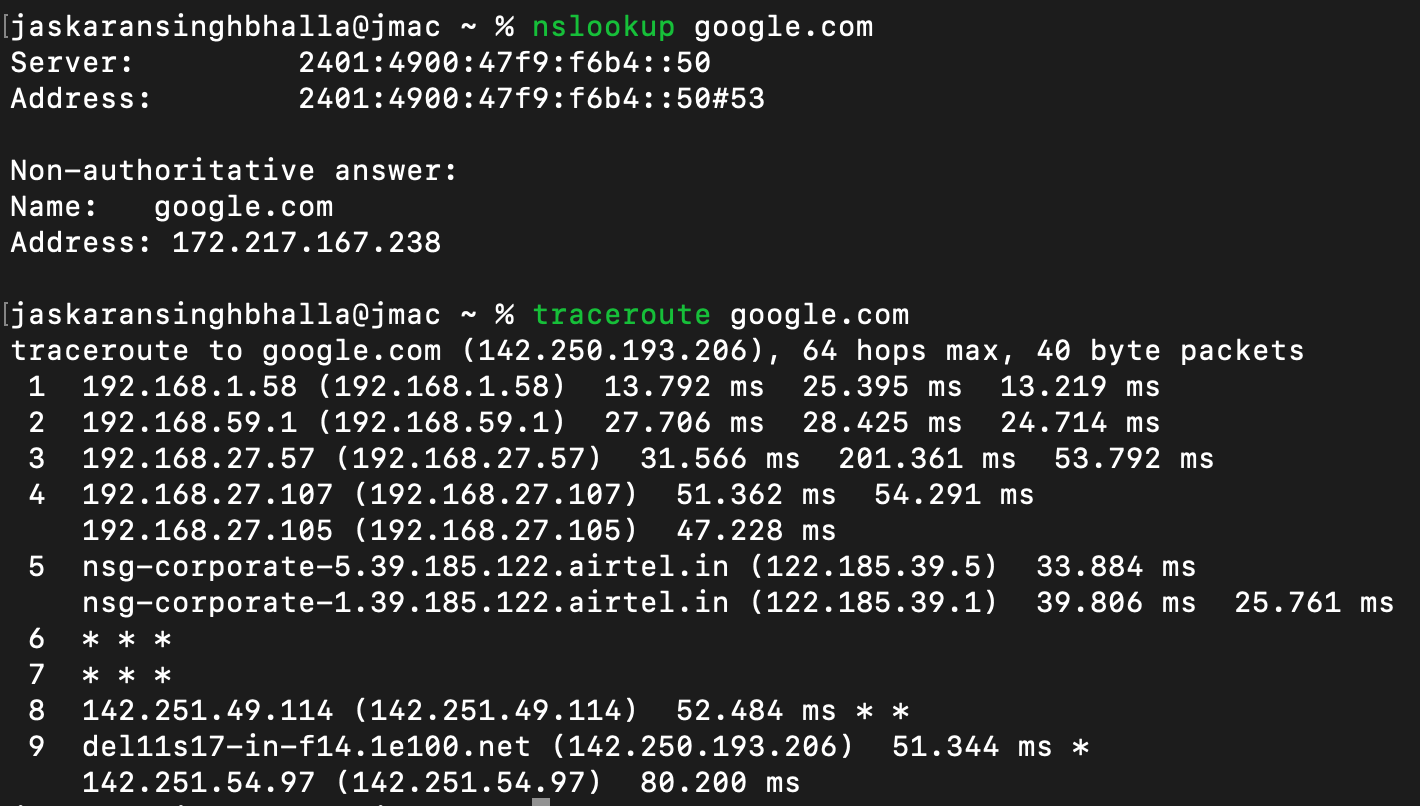
\includegraphics[width=\linewidth]{part-1/traceroute-celluar-google.png}
        \caption{Cellular Network using Hotspot}
    \end{minipage}
\end{figure}

\subsubsection*{Sigcomm.org}

\begin{figure}[H]
    \centering
    \begin{minipage}{0.45\textwidth}
        \centering
        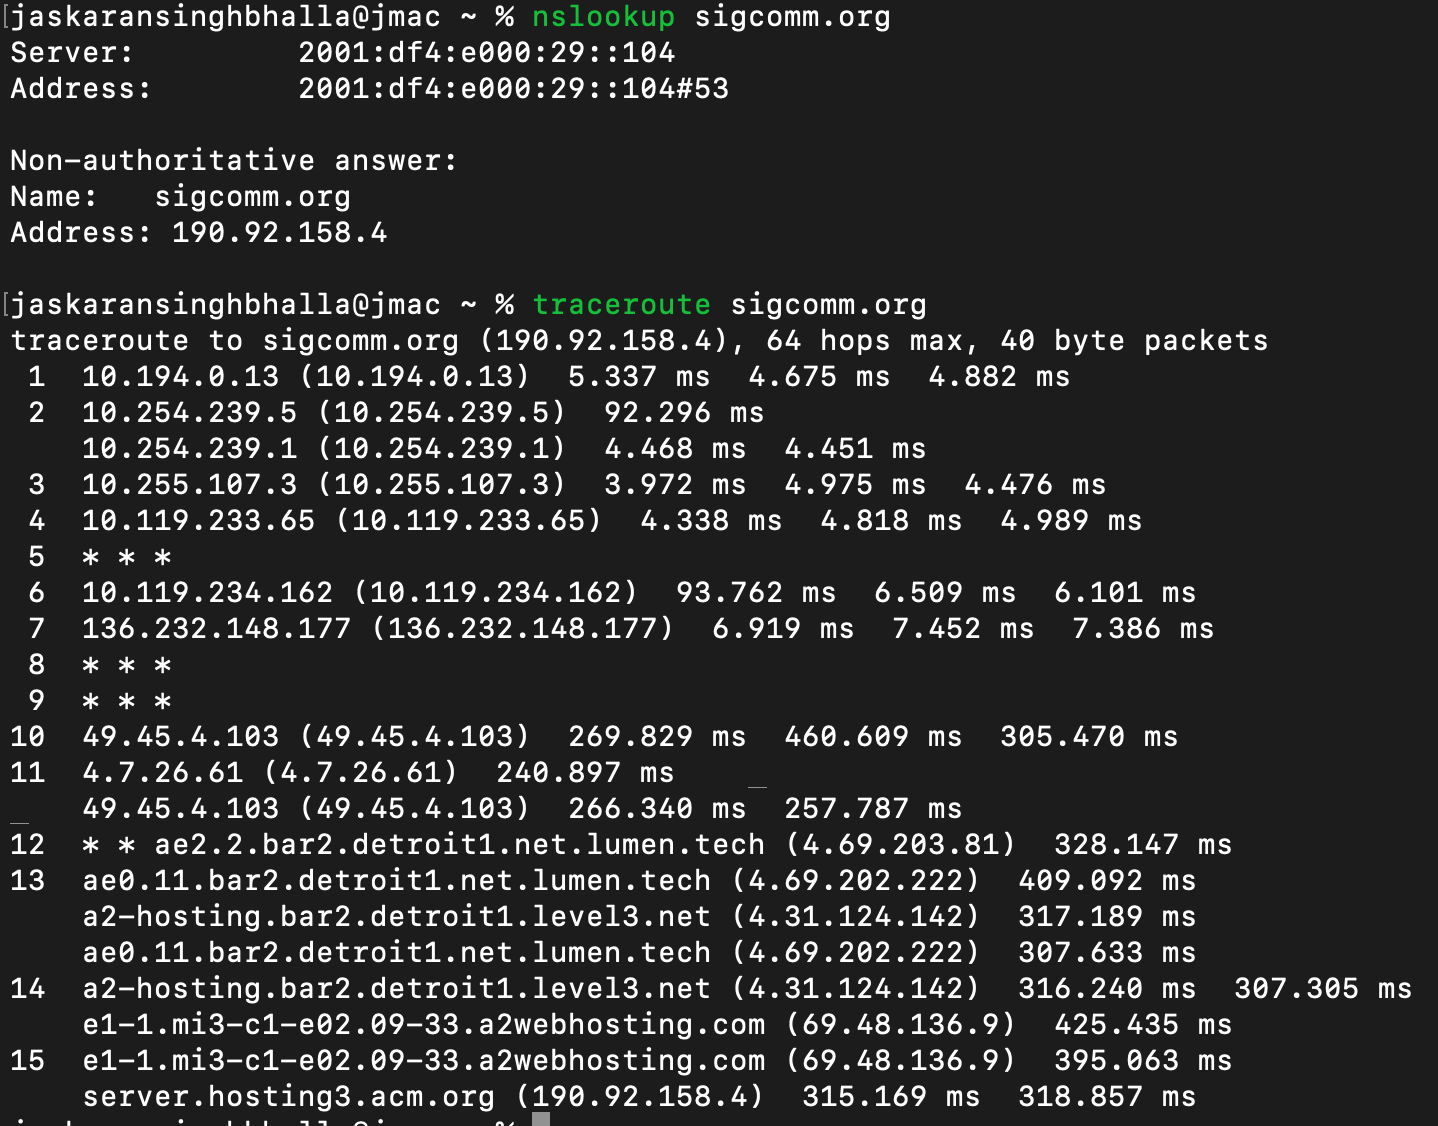
\includegraphics[width=\linewidth]{part-1/traceroute-iitd-sigcomm.png}
        \caption{IIT Delhi Network}
    \end{minipage}
    \hfill
    \begin{minipage}{0.45\textwidth}
        \centering
        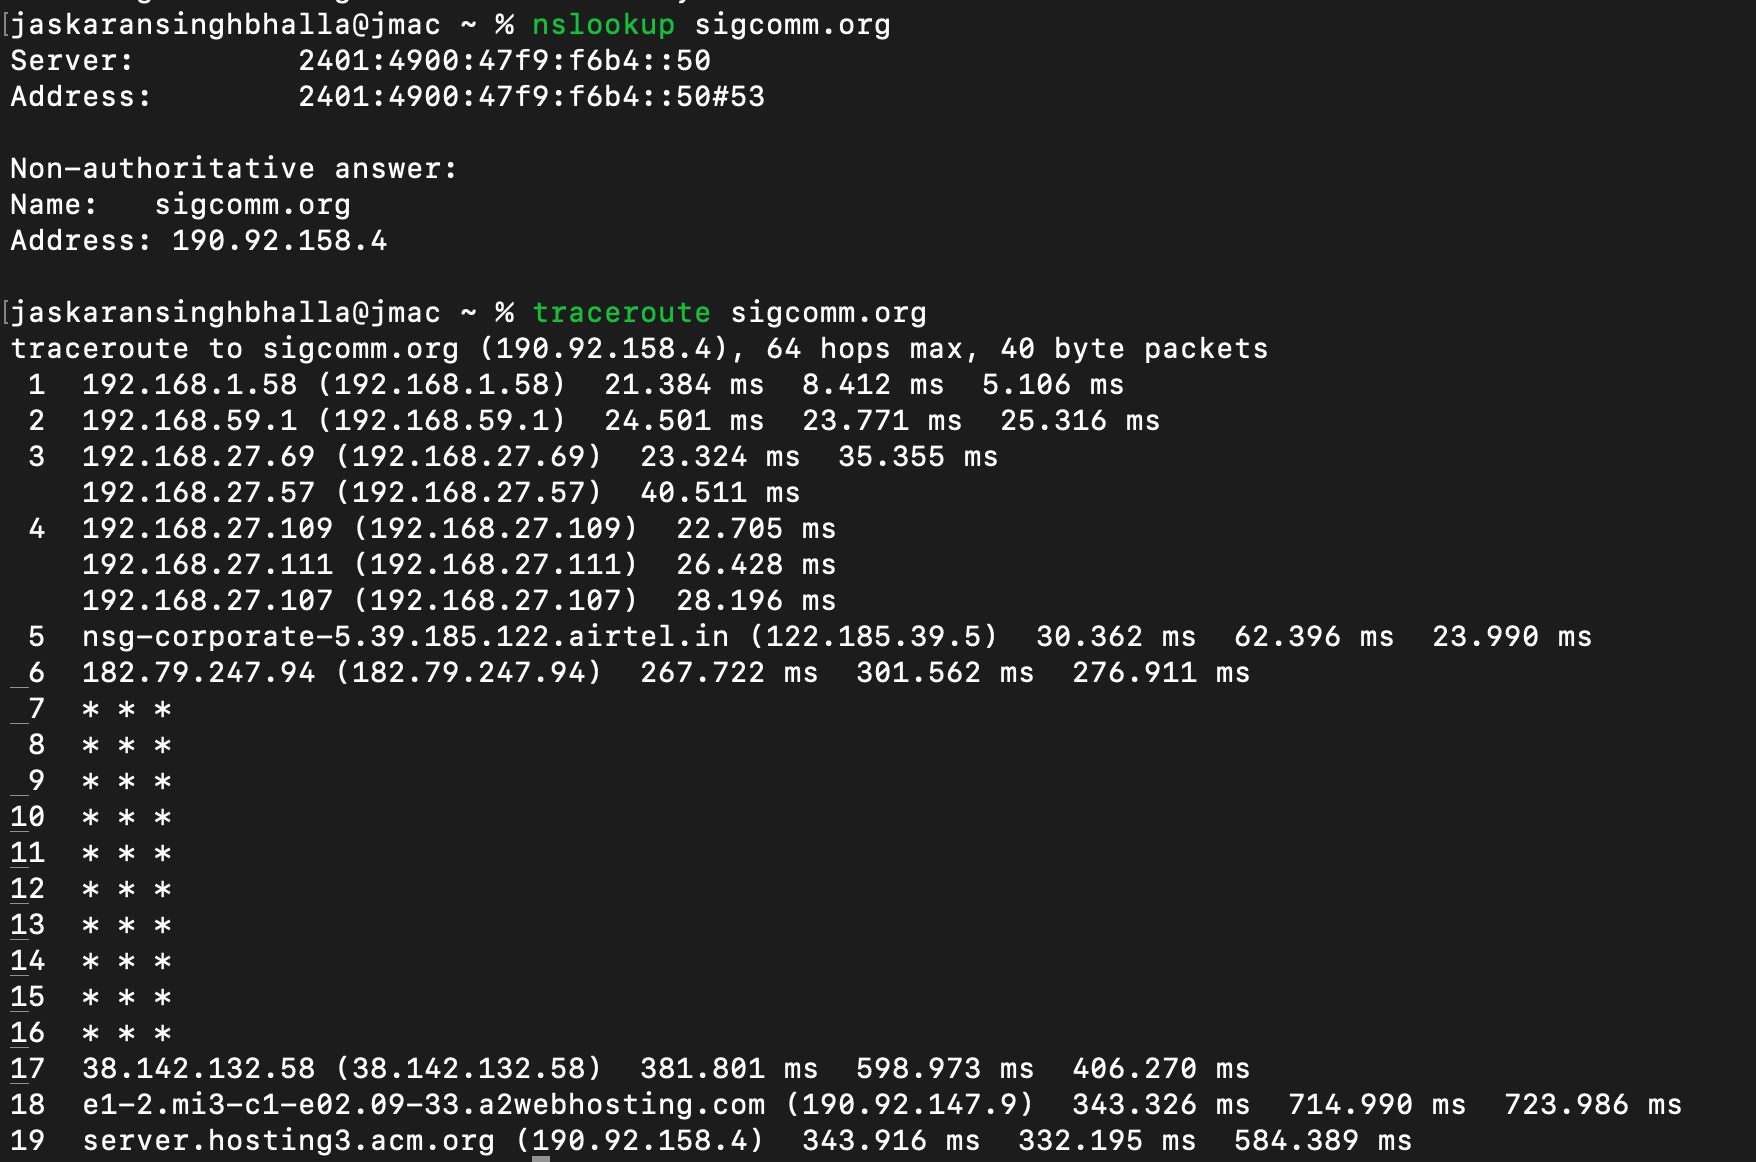
\includegraphics[width=\linewidth]{part-1/traceroute-celluar-sigcomm.png}
        \caption{Cellular Network using Hotspot}
    \end{minipage}
\end{figure}

\subsection{Number of hops and Autonomous systems}
\noindent
In computer networks, a hop refers to the journey of a packet of data from one router to another router, in travelling from source to destination. Number of hops is therefore an indicator of the number of routers, a data packet passes through in going from source to destination. Using \verb|traceroute| command we can calculate the number of hops by the line number that is logged. Each line with a number represents a single hop.

\noindent
So, the number of hops for google.com on IIT Delhi's network are 10 and on cellular network are 9. Similarly, for sigcomm.org, number of hops on IIT Delhi's network are 15 and on cellular network are 19.

\noindent
To list the number of autonomous systems observed we can use \verb|whois| command and look for origin or originAS code to get the AS number. For google.com on IIT Delhi's network and cellular network, we have list of AS = [AS15169]. It contains a single autonomous system. For sigcomm also we observed AS = [AS55293] on IIT Delhi's network and AS =[AS174, AS55293]. To compute this we ran \verb|whois| for each IP address inn the \verb|traceroute| output for both the networks.

\subsection{Asterisk (*) in output}
\noindent
Yes we observed Asterisk in the logs from \verb|traceroute| we got. They typically indicate a timeout response, which means that the probe packet sent to that particular hop did not return a response within the expected time frame. With reference we can have either of the three situations in which Asterisk appear

\noindent
\textbf{Single Asterisk on a Hop}: This means that the request timed out on just one of the three attempts. This can be a sign that there is an intermittent problem at that hop.

\noindent
\textbf{Three Asterisks, Then Failure}: If we see all three attempts at a hop have asterisks and then the traceroute errors out, it means that the hop is completely down.

\noindent
\textbf{Three Asterisks, Then Success}: If we see three attempts at a hop failing but then the rest of the traceroute continues without an issue, that is actually not a problem at all. This simply means that (as mentioned earlier), the device at that hop is configured not to respond to pings or traceroutes, so the attempt times out.

\subsection{Multiple IP addresses for same hop count}
\noindent
In a traceroute output, observing multiple IP addresses for the same hop is quite common and can be attributed to several factors. Routers often have multiple network interfaces, each with its own IP address, so a single router might appear with different IPs if it has more than one interface. Additionally, many networks use load balancing to distribute traffic across various paths. This means that traceroute might show different IP addresses for the same hop because packets are routed through different interfaces to balance the network load. Redundancy and failover mechanisms also play a role; networks are designed with backup paths to ensure reliability, so if a primary path fails, packets might take an alternate route, resulting in different IP addresses for the same hop. Hostname resolution can further contribute to this phenomenon, as a single hostname might resolve to multiple IP addresses, leading to various IPs appearing in the traceroute. Lastly, complex network configurations, particularly in large networks, might use different IP addresses for distinct types of traffic or network segments. These factors, combined, reflect the sophisticated and resilient design of modern network infrastructures.


\subsection{Internet Architecture on traceroute}

\noindent
If we look at the list of IP addresses hopped for all four <network, website> combinations,. We find "10.194.0.13", "10.254.239.5", "10.254.239.1", "10.255.107.3", "10.119.233.65", and "10.119.234.162" are common routes hopped when we use both websites using the IIT Delhi network. Certainly, this means that these routes belong to IIT Delhi's network. Similarly, for a common cellular network, "192.168.1.58", "192.168.59.1", and "192.168.27.57" are common, indicating the local internet service provider. These routes therefore represent the lowest internet provider in the Internet architecture. 

\noindent 
We get the IP addresses on IIT Delhi's network for google.com as follows: "72.14.195.56", "142.251.226.85", "192.178.83.243", "142.251.76.169", "142.251.76.171", "142.250.207.206" These IP address give "Google LLC" on running \verb|whois| command and checking the OrgName attribute. This means that these servers are belong to Google, and we checked over Internet to find that these servers were owned by Google cloud computing. Similarly for cellular network the set of IP addresses traced are different "192.168.27.107", "192.168.27.105", "122.185.39.5", "122.185.39.1", "142.251.49.114", "142.250.193.206", "142.251.54.97" but they have the OrgName set to "Google LLC". This indicates the second level in the internet architecture for google.com. Google has 2-Tier architecture, where the local internet provide is directly connected to the Google's backbone internet.

\noindent
For sigcomm running \verb|whois| command on both the networks gave different providers. The end provider for this website is "A2 Hosting, Inc.". On cellular network we had two intermediate providers. One is an local network provider whose OrgName information was not visible. Then it hopped to a global ISP, who was also not traceable, Then it went to a American regional ISP "PSINet, Inc.", before reaching local ISP "A2 Hostings", which hosts sigcomm.org  So sigcomm followed a 3-Tier internet architecture on cellular network. On IIT Delhi's network we observed multiple hops from multiple providers. But the end provider was "A2 Hosting, Inc.". Intermediate providers included "Asia Pacific Network Info Center", "Level 3 Parent, LLC" owned by Lumen Technologies. Here we can see IIT Delhi's network is the local provider, ASNIC is the regional provider. Then it hopped from "49.45.4.103" which is the global Internet provider, "Level 3 Parent, LLC" is regional provider in America and "A2 Hosting, Inc." is another local provider. So this definitely shows a 3-tier internet architecture.

\subsection{Geo locating the IP address}
\subsubsection{Reverse DNS lookup}

\noindent
To find the Geo-location of the server using their IP address, we use \verb|curl ipinfo.io/$ip| for performing reverse DNS-lookup. For Google on cellular network, the network request goes to "Dadri, Uttar Pradesh", "Delhi, India". On IIT Delhi's network it originates from "Delhi, India" and then goes to "Deoli, India" and returns back to "Delhi, India". 

\noindent
For sigcomm.org, on cellular network the network request goes to "Dadri, Uttar Pradesh", "Chennai, Tamil Nadu", "South field, Michigan". On IIT Delhi's network the request goes from "Delhi, India", "Los Angeles, California", "Detroit, Michigan". 
% \subsubsection{Maxmind database for IP Geo-location}
\subsubsection{Comparison of Geo locations with RTTs}

\noindent
Since the geolocation of the server is very close to the origin of the request, it justifies our short duration of round trip time (RTT) of 11.858 ms and 345.405 ms.

\noindent
For sigcomm.org, as the final server is located far away in Michigan, US. This justifies a longer RTT for this website, which was 345.405 ms and 554,750 ms So this indicates that closer location of the server is to location of request being sent, less is the round trip time and faster is the response.

% \section{Network Data Collection and Header Analysis}
% Do in a separate Report
% \section{Network Traffic Analysis}
% Do in a separate Report

\end{document}